% 
\documentclass[a4paper]{article}\usepackage{graphicx, color}
%% maxwidth is the original width if it is less than linewidth
%% otherwise use linewidth (to make sure the graphics do not exceed the margin)
\makeatletter
\def\maxwidth{ %
  \ifdim\Gin@nat@width>\linewidth
    \linewidth
  \else
    \Gin@nat@width
  \fi
}
\makeatother

\IfFileExists{upquote.sty}{\usepackage{upquote}}{}
\definecolor{fgcolor}{rgb}{0.2, 0.2, 0.2}
\newcommand{\hlnumber}[1]{\textcolor[rgb]{0,0,0}{#1}}%
\newcommand{\hlfunctioncall}[1]{\textcolor[rgb]{0.501960784313725,0,0.329411764705882}{\textbf{#1}}}%
\newcommand{\hlstring}[1]{\textcolor[rgb]{0.6,0.6,1}{#1}}%
\newcommand{\hlkeyword}[1]{\textcolor[rgb]{0,0,0}{\textbf{#1}}}%
\newcommand{\hlargument}[1]{\textcolor[rgb]{0.690196078431373,0.250980392156863,0.0196078431372549}{#1}}%
\newcommand{\hlcomment}[1]{\textcolor[rgb]{0.180392156862745,0.6,0.341176470588235}{#1}}%
\newcommand{\hlroxygencomment}[1]{\textcolor[rgb]{0.43921568627451,0.47843137254902,0.701960784313725}{#1}}%
\newcommand{\hlformalargs}[1]{\textcolor[rgb]{0.690196078431373,0.250980392156863,0.0196078431372549}{#1}}%
\newcommand{\hleqformalargs}[1]{\textcolor[rgb]{0.690196078431373,0.250980392156863,0.0196078431372549}{#1}}%
\newcommand{\hlassignement}[1]{\textcolor[rgb]{0,0,0}{\textbf{#1}}}%
\newcommand{\hlpackage}[1]{\textcolor[rgb]{0.588235294117647,0.709803921568627,0.145098039215686}{#1}}%
\newcommand{\hlslot}[1]{\textit{#1}}%
\newcommand{\hlsymbol}[1]{\textcolor[rgb]{0,0,0}{#1}}%
\newcommand{\hlprompt}[1]{\textcolor[rgb]{0.2,0.2,0.2}{#1}}%

\usepackage{framed}
\makeatletter
\newenvironment{kframe}{%
 \def\at@end@of@kframe{}%
 \ifinner\ifhmode%
  \def\at@end@of@kframe{\end{minipage}}%
  \begin{minipage}{\columnwidth}%
 \fi\fi%
 \def\FrameCommand##1{\hskip\@totalleftmargin \hskip-\fboxsep
 \colorbox{shadecolor}{##1}\hskip-\fboxsep
     % There is no \\@totalrightmargin, so:
     \hskip-\linewidth \hskip-\@totalleftmargin \hskip\columnwidth}%
 \MakeFramed {\advance\hsize-\width
   \@totalleftmargin\z@ \linewidth\hsize
   \@setminipage}}%
 {\par\unskip\endMakeFramed%
 \at@end@of@kframe}
\makeatother

\definecolor{shadecolor}{rgb}{.97, .97, .97}
\definecolor{messagecolor}{rgb}{0, 0, 0}
\definecolor{warningcolor}{rgb}{1, 0, 1}
\definecolor{errorcolor}{rgb}{1, 0, 0}
\newenvironment{knitrout}{}{} % an empty environment to be redefined in TeX

\usepackage{alltt}
%\usepackage{Sweave}
%\SweaveOpts{keep.source=TRUE}

%\usepackage[OT1]{fontenc}
\usepackage[colorlinks]{hyperref}
\usepackage{a4wide}
\usepackage{xspace}
\usepackage[all]{hypcap} % for linking to the top of the figures or tables

% add preamble from pkgmaker
%%%% PKGMAKER COMMANDS %%%%%%
\usepackage{xspace}

% R
\let\proglang=\textit
\let\code=\texttt 
\newcommand{\Rcode}{\code}
\newcommand{\pkgname}[1]{\textit{#1}\xspace}
\newcommand{\Rpkg}[1]{\pkgname{#1} package\xspace}
\newcommand{\citepkg}[1]{\cite{#1}}

% CRAN
\newcommand{\CRANurl}[1]{\url{http://cran.r-project.org/package=#1}}
%% CRANpkg
\makeatletter
\def\CRANpkg{\@ifstar\@CRANpkg\@@CRANpkg}
\def\@CRANpkg#1{\href{http://cran.r-project.org/package=#1}{\pkgname{#1}}\footnote{\CRANurl{#1}}}
\def\@@CRANpkg#1{\href{http://cran.r-project.org/package=#1}{\pkgname{#1}} package\footnote{\CRANurl{#1}}}
\makeatother
%% citeCRANpkg
\makeatletter
\def\citeCRANpkg{\@ifstar\@citeCRANpkg\@@citeCRANpkg}
\def\@citeCRANpkg#1{\CRANpkg{#1}\cite*{Rpackage:#1}}
\def\@@citeCRANpkg#1{\CRANpkg{#1}~\cite{Rpackage:#1}}
\makeatother
\newcommand{\CRANnmf}{\href{http://cran.r-project.org/package=NMF}{CRAN}}
\newcommand{\CRANnmfURL}{\url{http://cran.r-project.org/package=NMF}}

% Bioconductor
\newcommand{\BioCurl}[1]{\url{http://www.bioconductor.org/packages/release/bioc/html/#1.html}}
\newcommand{\BioCpkg}[1]{\href{http://www.bioconductor.org/packages/release/bioc/html/#1.html}{\pkgname{#1}} package\footnote{\BioCurl{#1}}}
\newcommand{\citeBioCpkg}[1]{\BioCpkg{#1}~\cite{Rpackage:#1}}
% Bioconductor annotation
\newcommand{\BioCAnnurl}[1]{\url{http://www.bioconductor.org/packages/release/data/annotation/html/#1.html}}
\newcommand{\BioCAnnpkg}[1]{\href{http://www.bioconductor.org/packages/release/data/annotation/html/#1.html}{\Rcode{#1}} annotation package\footnote{\BioCAnnurl{#1}}}
\newcommand{\citeBioCAnnpkg}[1]{\BioCAnnpkg{#1}~\cite{Rpackage:#1}}

% GEO
\newcommand{\GEOurl}[1]{\href{http://www.ncbi.nlm.nih.gov/geo/query/acc.cgi?acc=#1}{#1}\xspace}
\newcommand{\GEOhref}[1]{\GEOurl{#1}\footnote{\url{http://www.ncbi.nlm.nih.gov/geo/query/acc.cgi?acc=#1}}}

% ArrayExpress
\newcommand{\ArrayExpressurl}[1]{\href{http://www.ebi.ac.uk/arrayexpress/experiments/#1}{#1}\xspace}
\newcommand{\ArrayExpresshref}[1]{\ArrayExpressurl{#1}\footnote{\url{http://www.ebi.ac.uk/arrayexpress/experiments/#1}}}

%%%% END: PKGMAKER COMMANDS %%%%%%



\newcommand{\nmfpack}{\pkgname{NMF}}
\newcommand{\MATLAB}{MATLAB\textsuperscript{\textregistered}\xspace}
\newcommand{\refeqn}[1]{(\ref{#1})}

% REFERENCES
\usepackage[citestyle=authoryear-icomp
, doi=true
, url=true
, maxnames=1
, maxbibnames=15
, backref=true]{biblatex}
\AtEveryCitekey{\clearfield{url}}
\bibliography{/tmp/Rpkglib_4373a6292f/NMF/REFERENCES}


\bibliography{Rpackages}
\newcommand{\citet}[1]{\textcite{#1}}
\renewcommand{\cite}[1]{\parencite{#1}}
\DefineBibliographyStrings{english}{%
    backrefpage  = {see p.}, % for single page number
    backrefpages = {see pp.} % for multiple page numbers
}
%

% boxed figures
\usepackage{float}
\floatstyle{boxed} 
\restylefloat{figure}

\usepackage{array}
\usepackage{tabularx}
\usepackage{mathabx}

\usepackage{url}
\urlstyle{rm}

% use cleveref for automatic reference label formatting
\usepackage[capitalise, noabbrev]{cleveref}

% define commands for notes
\usepackage{todonotes}
\newcommand{\nbnote}[1]{\ \bigskip\todo[inline, backgroundcolor=blue!20!white]{\scriptsize\textsf{\textbf{NB:} #1}}\ \\}

% put table of contents on two columns
\usepackage[toc]{multitoc}

\setkeys{Gin}{width=0.95\textwidth}

\begin{document}




\title{Generating heatmaps for Nonnegative Matrix Factorization\\
\small Package \nmfpack\ - Version 0.11}
\author{Renaud Gaujoux}
% \VignetteIndexEntry{NMF: generating heatmaps}
% \VignetteDepends{NMF,RColorBrewer}
% \VignetteKeyword{aplot}
% \VignetteCompiler{knitr}

\maketitle

\begin{abstract}
This vignette describes how to produce different informative heatmaps from NMF objects, 
such as returned by the function \code{nmf} in the \citeCRANpkg{NMF}.
The main drawing engine is implemented by the function \code{aheatmap}, which is 
a highly enhanced modification of the function \code{pheatmap} from the \citeCRANpkg{pheatmap},
and provides convenient and quick ways of producing high quality and customizable annotated heatmaps.
Currently this function is part of the package \nmfpack, but may eventually 
compose a separate package on its own.
\end{abstract}

{\small \tableofcontents}

\section{Preliminaries}

\subsection{Quick reminder on NMF models}

Given a nonnegative target matrix $X$ of dimension $n\times p$, NMF algorithms 
aim at finding a rank $k$ approximation of the form:
$$
X \approx W H,
$$
where $W$ and $H$ are nonnegative matrices of dimensions $n\times k$ and $k\times p$ 
respectively.

The matrix $W$ is the basis matrix, whose columns are the basis components.
The matrix $H$ is the mixture coefficient or weight matrix, whose columns contain 
the contribution of each basis component to the corresponding column of $X$.
We call the rows of $H$ the basis profiles.

\subsection{Heatmaps for NMF}

Because NMF objects essentially wrap up a pair of matrices, heatmaps are convenient 
to visualise the results of NMF runs. 
The package \nmfpack provides several specialised heatmap functions, designed to produce 
heatmaps with sensible default configurations according to the data being drawn.
Being all based on a common drawing engine, they share almost identical interfaces 
and capabilities.
The following specialised functions are currently implemented:

\begin{description}
\item[\code{basismap}] draws heatmaps of the basis matrix 
\item[\code{coefmap}] draws heatmaps of the mixture coefficient matrix
\item[\code{consensusmap}] draws heatmaps of the consensus matrix, for results 
of multiple NMF runs.
\end{description}

\subsection{Heatmap engine}

All the above functions eventually call a common heatmap engine, with 
different default parameters, chosen to be relevant for the given underlying data.
The engine is implemented by the function \code{aheatmap}. 
Its development started as modification of the function \code{pheatmap} from 
the \pkgname{pheatmap} package. 
The initial objective was to improve and increase its capabilities, as well as 
defining a simplified interface, more consistent with the R core function \code{heatmap}.
We eventually aim at providing a general, flexible, powerful and easy to use engine 
for drawing annotated heatmaps.
  
The function \code{aheatmap} has many advantages compared to other heatmap functions 
such as \code{heatmap}, \code{gplots::heatmap2}, \code{heatmap.plus::heatmap.plus} 
, or even \code{pheatmap}:

\begin{itemize}
\item Annotations: unlimited number of annotation tracks can be added to 
\emph{both} columns and rows, with automated colouring for categorical and 
numeric variables.
\item Compatibility with both base and grid graphics: the function can be 
directly called in drawing contexts such as grid, mfrow or layout.
This is a feature many R users were looking for, and that was strictly 
impossible with base heatmaps.
\item Legends: default automatic legend and colouring;
\item Customisation: clustering methods, annotations, colours and legend can all 
be customised, even separately for rows and columns;
\item Convenient interface: many arguments provide multiple ways of 
specifying their value(s), which speeds up developping/writing and reduce the 
amount of code required to generate customised plots (e.g. see
\cref{sec:colour_spec}).
\item Aesthetics: the heatmaps look globally cleaner, the image and text components 
are by default well proportioned relatively to each other, and all fit within 
the graphic device.
\end{itemize}

\subsection{Data and model}
\label{sec:data}

For the purpose of illustrating the use of each heatmap function, we generate a 
random target matrix, as well as some annotations or covariates:

\begin{knitrout}
\definecolor{shadecolor}{rgb}{0.969, 0.969, 0.969}\color{fgcolor}\begin{kframe}
\begin{alltt}
\hlcomment{# random data that follow an 3-rank NMF model (with quite some noise:}
\hlcomment{# sd=2)}
X <- \hlfunctioncall{syntheticNMF}(100, 3, 20, noise = 2)

\hlcomment{# row annotations and covariates}
n <- \hlfunctioncall{nrow}(X)
d <- \hlfunctioncall{rnorm}(n)
e <- \hlfunctioncall{unlist}(\hlfunctioncall{mapply}(rep, \hlfunctioncall{c}(\hlstring{"X"}, \hlstring{"Y"}, \hlstring{"Z"}), 10))
e <- \hlfunctioncall{c}(e, \hlfunctioncall{rep}(NA, n - \hlfunctioncall{length}(e)))
rdata <- \hlfunctioncall{data.frame}(Var = d, Type = e)

\hlcomment{# column annotations and covariates}
p <- \hlfunctioncall{ncol}(X)
a <- \hlfunctioncall{sample}(\hlfunctioncall{c}(\hlstring{"alpha"}, \hlstring{"beta"}, \hlstring{"gamma"}), p, replace = TRUE)
\hlcomment{# define covariates: true groups and some numeric variable}
c <- \hlfunctioncall{rnorm}(p)
\hlcomment{# gather them in a data.frame}
covariates <- \hlfunctioncall{data.frame}(a, X$pData, c)
\end{alltt}
\end{kframe}
\end{knitrout}


%\SweaveOpts{fig.width=14,fig.height=7}


Note that in the code above, the object \code{X} returned by \code{syntheticNMF} \emph{really is} a matrix object, but wrapped through the function \code{ExposedAttribute} object, which exposes its attributes via a more friendly and access controlled interface \code{\$}.
Of particular interests are attributes \code{'pData'} and \code{'fData'}, which are lists that contain a factor named \code{'Group'} that indicates the true underlying clusters.
These are respectively defined as each sample's most contrbuting basis component and the basis component to which each feature contributes the most.
They are useful to annotate heatmaps and assess the ability of NMF methods to recover the true clusters. 

As an example, one can conveniently visualize the target matrix as a heatmap, with or without the relevant sample and feature annotations, using simple calls to the \code{aheatmap} function:
\begin{knitrout}
\definecolor{shadecolor}{rgb}{0.969, 0.969, 0.969}\color{fgcolor}\begin{kframe}
\begin{alltt}
\hlfunctioncall{par}(mfrow = \hlfunctioncall{c}(1, 2))
\hlfunctioncall{aheatmap}(X, annCol = covariates, annRow = X$fData)
\hlfunctioncall{aheatmap}(X)
\end{alltt}
\end{kframe}
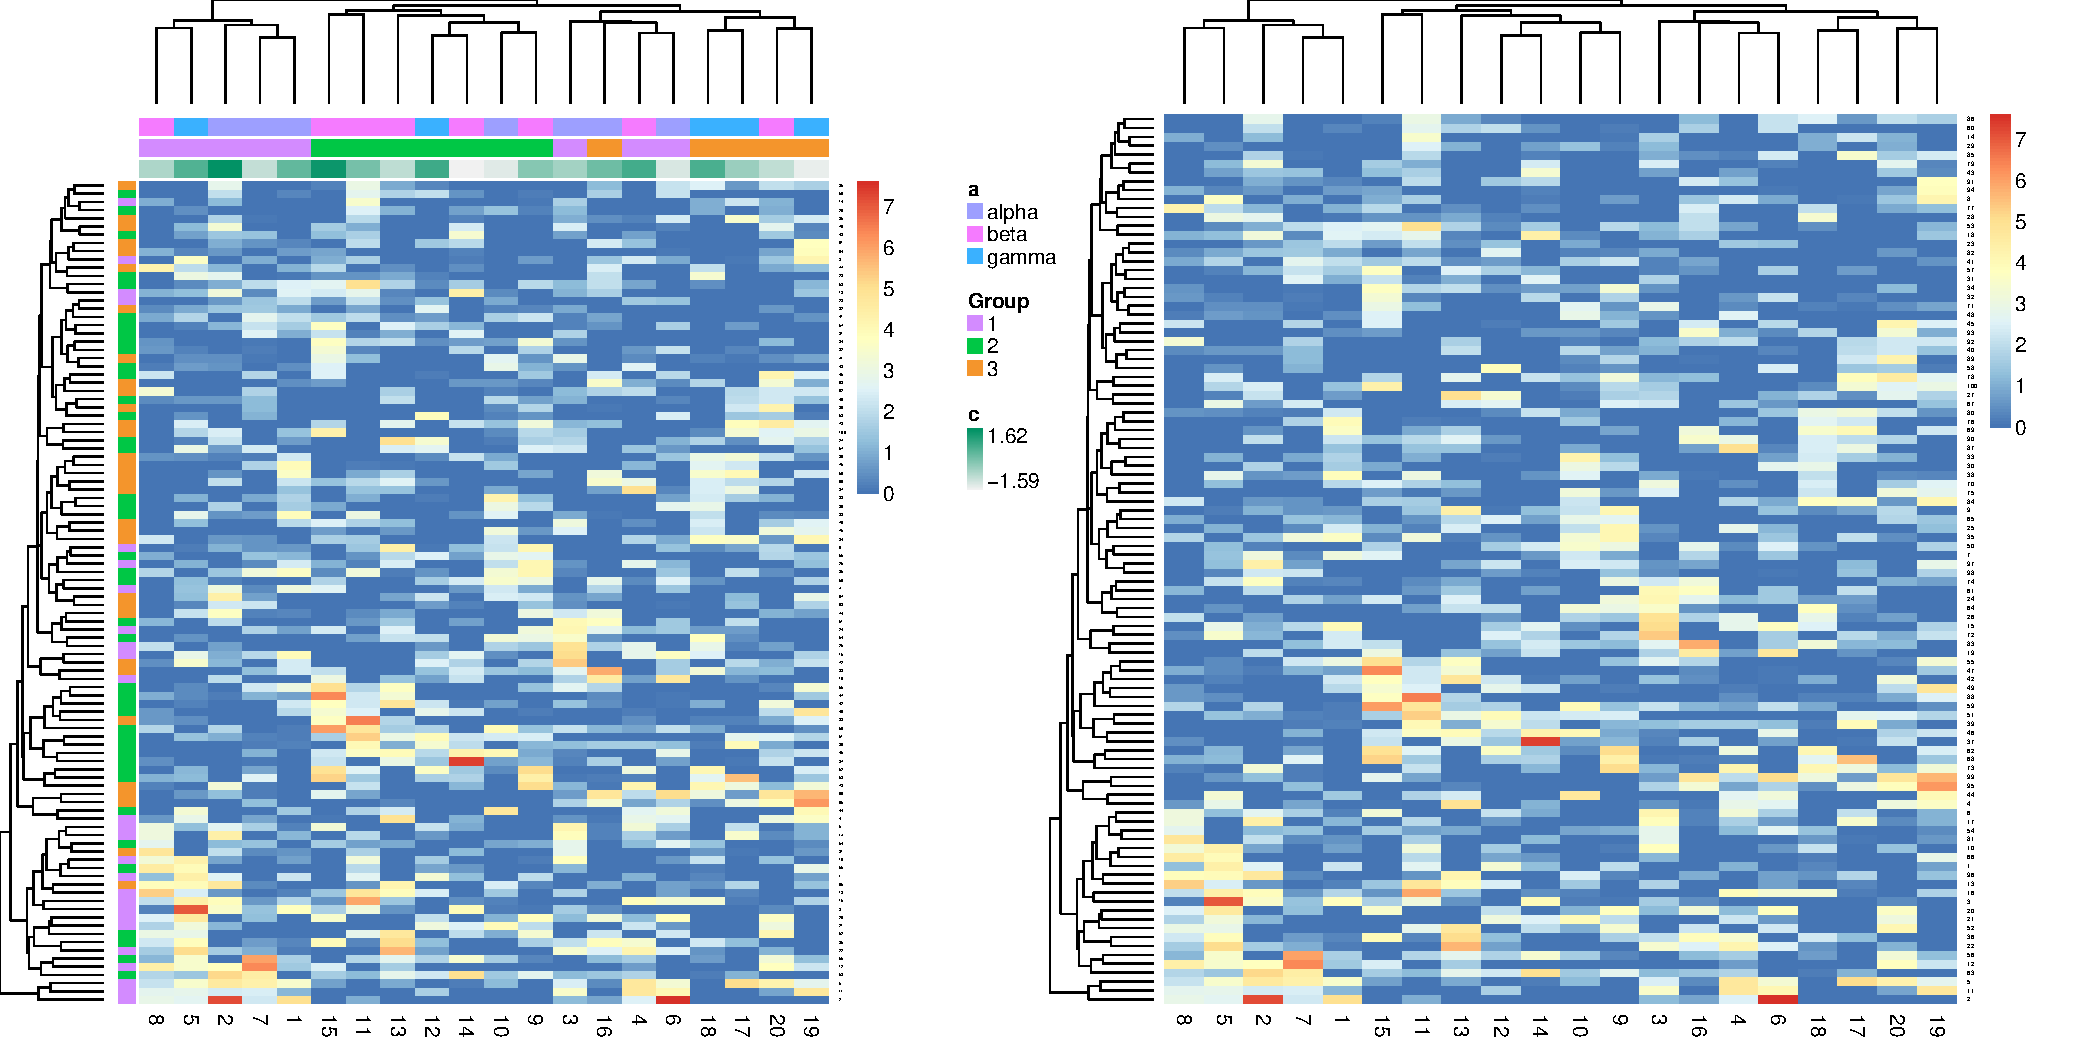
\includegraphics[width=\maxwidth]{/home/renaud/Documents/projects/NMF/pkg/vignettes/figure/heatmaps-heatmap_data} 

\end{knitrout}


Then, we fit an NMF model using multiple runs, that will be used throughtout this vignette to illustrate the use of NMF heatmaps:

\begin{knitrout}
\definecolor{shadecolor}{rgb}{0.969, 0.969, 0.969}\color{fgcolor}\begin{kframe}
\begin{alltt}
res <- \hlfunctioncall{nmf}(X, 3, nrun = 10)
res
\end{alltt}
\begin{verbatim}
## <Object of class: NMFfitX1 >
##   Method: brunet 
##   Runs:  10 
##   RNG:
##    407L, 1836648330L, -690549885L, 21815016L, -792180791L, -1546669834L, 1782788863L 
##   Total timing:
##    user  system elapsed 
##   3.520   0.204   1.889
\end{verbatim}
\end{kframe}
\end{knitrout}


\nbnote{To keep the vignette simple, we always use the default NMF method 
(i.e. \code{'brunet'}), but all steps could be performed using a different method, 
or multiple methods in order to compare their perfromances.}

\section{Mixture Coefficient matrix: \texttt{coefmap}}

The coefficient matrix of the result can be plotted using the function
\code{coefmap}.
The default behaviour for multiple NMF runs is to add two annotation tracks that 
show the clusters obtained by the best fit and the hierarchical clustering of 
the consensus matrix\footnote{The hierarchical clustering is computed using the 
consensus matrix itself as a similarity measure, and average linkage. See
\code{?consensushc}.}.
In the legend, these tracks are named \emph{basis} and \emph{consensus} respectively.
For single NMF run or NMF model objects, no consensus data are available, and 
only the clusters from the fit are displayed.

\begin{knitrout}
\definecolor{shadecolor}{rgb}{0.969, 0.969, 0.969}\color{fgcolor}\begin{kframe}
\begin{alltt}
opar <- \hlfunctioncall{par}(mfrow = \hlfunctioncall{c}(1, 2))
\hlcomment{# coefmap from multiple run fit: includes a consensus track}
\hlfunctioncall{coefmap}(res)
\hlcomment{# coefmap of a single run fit: no consensus track}
\hlfunctioncall{coefmap}(\hlfunctioncall{minfit}(res))
\end{alltt}
\end{kframe}
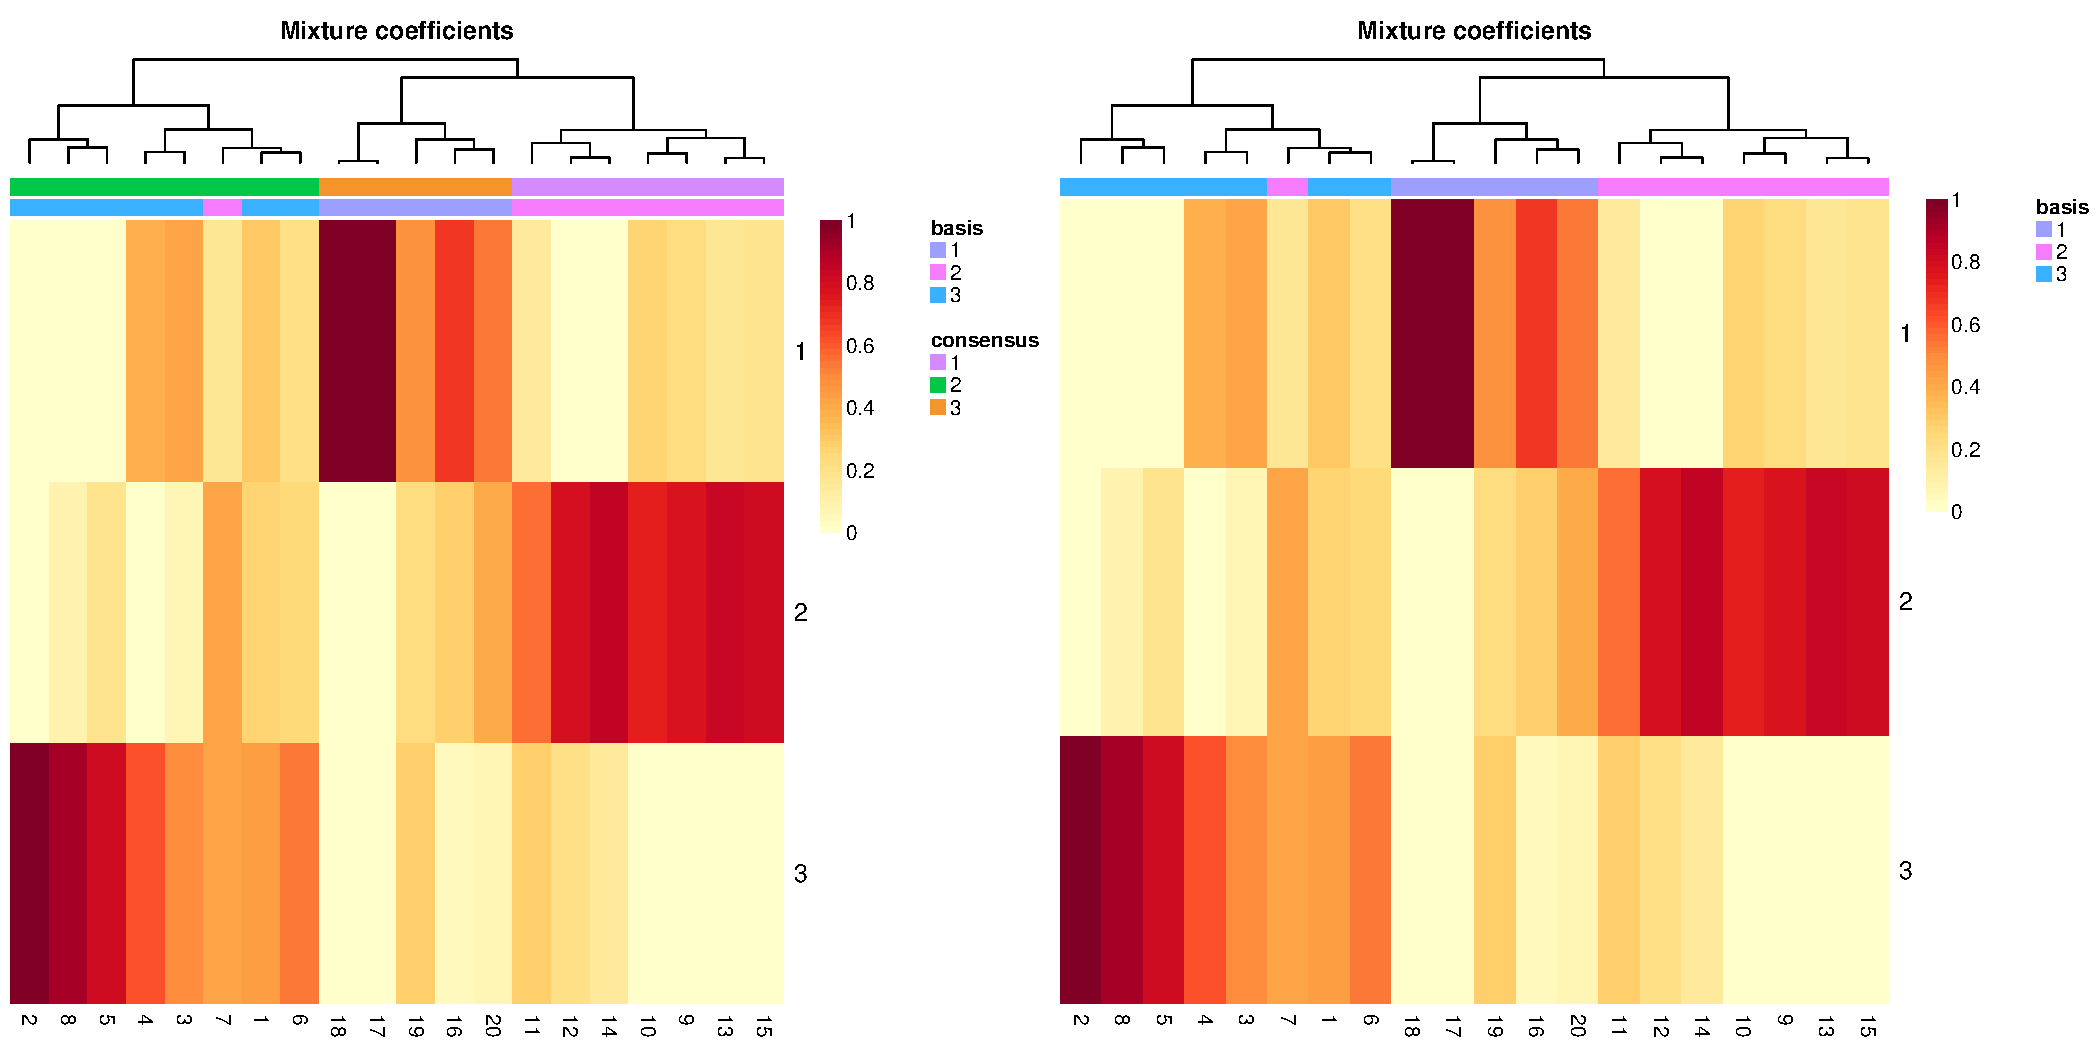
\includegraphics[width=\maxwidth]{/home/renaud/Documents/projects/NMF/pkg/vignettes/figure/heatmaps-coefmap_res} 
\begin{kframe}\begin{alltt}
\hlfunctioncall{par}(opar)
\end{alltt}
\end{kframe}
\end{knitrout}


\nbnote{Note how both heatmaps were drawn on the same plot, simply using the standard 
call to \code{par(mfrow=c(1,2)}.
This is impossible to achieve with the R core function \code{heatmap}.
See \cref{sec:aheatmap} for more details about compatibility with base 
and grid graphics.}

By default:
\begin{itemize}
\item the rows are not ordered;
\item the columns use the default ordering of \code{aheatmap}, but may easily be
ordered according to the clusters defined by the dominant basis component for 
each column with \code{Colv="basis"}, or according to those implied by the
consensus matrix, i.e. as in \code{consensusmap}, with \code{Colv="consensus"};
\item each column is scaled to sum up to one;
\item the color palette used is \code{'YlOrRd'} from the
\citeCRANpkg{RColorBrewer}, with 50 breaks.
\end{itemize}

In term of arguments passed to the heatmap engine \code{aheatmap}, these default 
settings translate as:

\begin{knitrout}
\definecolor{shadecolor}{rgb}{0.969, 0.969, 0.969}\color{fgcolor}\begin{kframe}
\begin{alltt}
Rowv = NA
Colv = TRUE
scale = \hlstring{"c1"}
color = \hlstring{"YlOrRd:50"}
annCol = \hlfunctioncall{predict}(object) + \hlfunctioncall{predict}(object, \hlstring{"consensus"})
\end{alltt}
\end{kframe}
\end{knitrout}


If the ordering does not come from a hierarchical clustering (e.g., if
\code{Colv='basis'}), then no dendrogram is displayed.
The default behaviour of \code{aheatmap} can be obtained by setting arguments 
\code{Rowv=TRUE, Colv=TRUE, scale='none'}.

\medskip
The automatic annotation tracks can be hidden all together by setting argument 
\code{tracks=NA}, displayed separately by passing only one of the given names 
(e.g. \code{tracks=':basis'} or \code{tracks='basis:'} for the row or column respectively),
and their legend names may be changed by
specifying e.g. \code{tracks=c(Metagene=':basis', 'consensus')}.
Beside this, they are handled by the heatmap engine function \code{aheatmap} 
and can be customised as any other annotation tracks -- that can be added via 
the same argument \code{annCol} (see \cref{sec:aheatmap} or \code{?aheatmap} for
more details).

\begin{knitrout}
\definecolor{shadecolor}{rgb}{0.969, 0.969, 0.969}\color{fgcolor}\begin{kframe}
\begin{alltt}
opar <- \hlfunctioncall{par}(mfrow=\hlfunctioncall{c}(1,2))
\hlcomment{# removing all automatic annotation tracks}
\hlfunctioncall{coefmap}(res, tracks=NA)
\hlcomment{# customized plot}
\hlfunctioncall{coefmap}(res, Colv = \hlstring{'euclidean'}
	, main = \hlstring{"Metagene contributions in each sample"}, labCol = NULL
	, annRow = \hlfunctioncall{list}(Metagene=\hlstring{':basis'}), annCol = \hlfunctioncall{list}(\hlstring{':basis'}, Class=a, Index=c)
	, annColors = \hlfunctioncall{list}(Metagene=\hlstring{'Set2'})
	, info = TRUE)
\end{alltt}
\end{kframe}
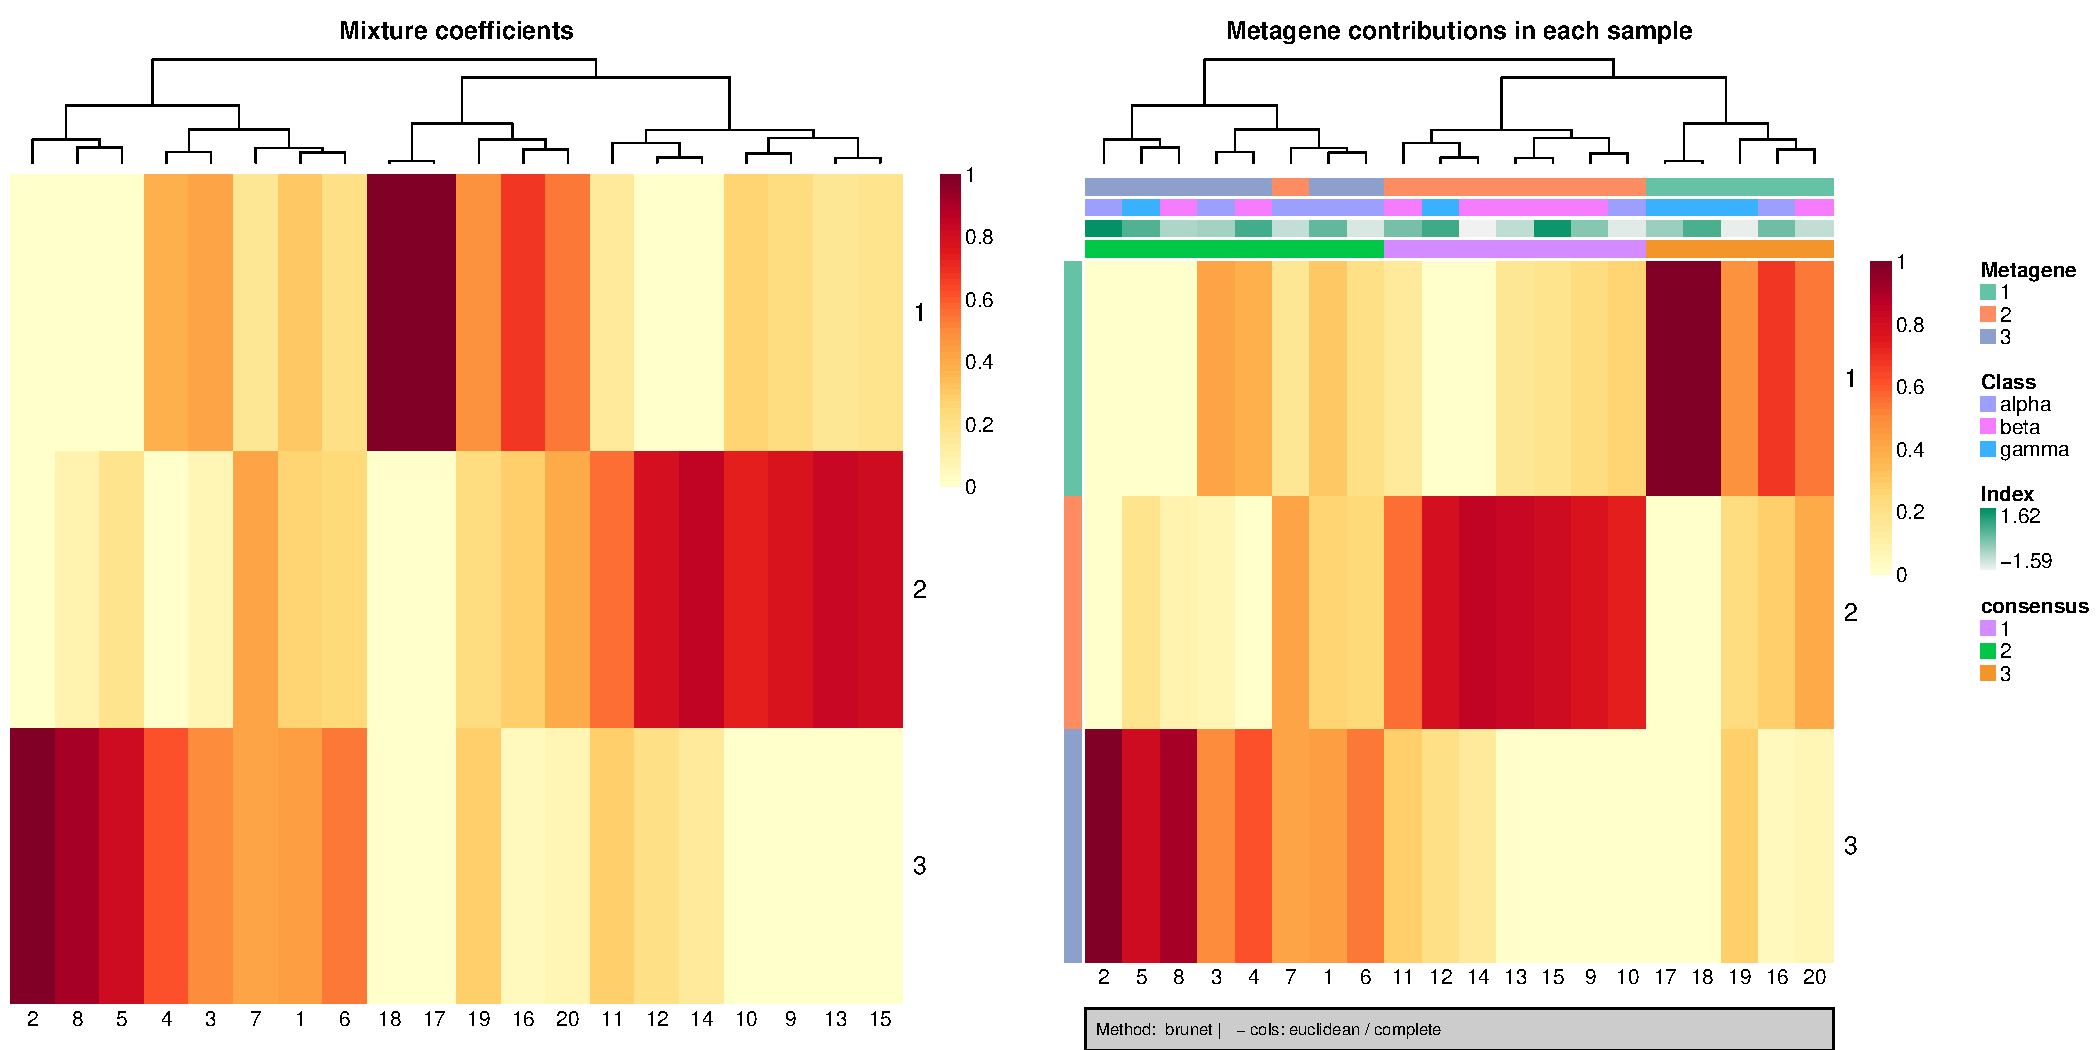
\includegraphics[width=\maxwidth]{/home/renaud/Documents/projects/NMF/pkg/vignettes/figure/heatmaps-coefmap_custom} 
\begin{kframe}\begin{alltt}
\hlfunctioncall{par}(opar)
\end{alltt}
\end{kframe}
\end{knitrout}


\nbnote{The feature that allows to display some information about the fit 
at the bottom of the plot via argument \code{info=TRUE} is still experimental.
It is helpful mostly when developing algorithms or doing an analysis, but 
would seldom be used in publications.}

\section{Basis matrix: \texttt{basismap}}

The basis matrix can be plotted using the function \code{basismap}. 
The default behaviour is to add an annotation track that shows for each row 
the dominant basis component.
That is, for each row, the index of the basis component with the highest 
loading.

This track can be disabled by setting \code{tracks=NA}, and extra 
row annotations can be added using the same argument \code{annRow}.

\begin{knitrout}
\definecolor{shadecolor}{rgb}{0.969, 0.969, 0.969}\color{fgcolor}\begin{kframe}
\begin{alltt}
opar <- \hlfunctioncall{par}(mfrow = \hlfunctioncall{c}(1, 2))
\hlcomment{# default plot}
\hlfunctioncall{basismap}(res)
\hlcomment{# customized plot: only use row special annotation track.}
\hlfunctioncall{basismap}(res, main = \hlstring{"Metagenes"}, annRow = \hlfunctioncall{list}(d, e), tracks = \hlfunctioncall{c}(Metagene = \hlstring{":basis"}))
\end{alltt}
\end{kframe}
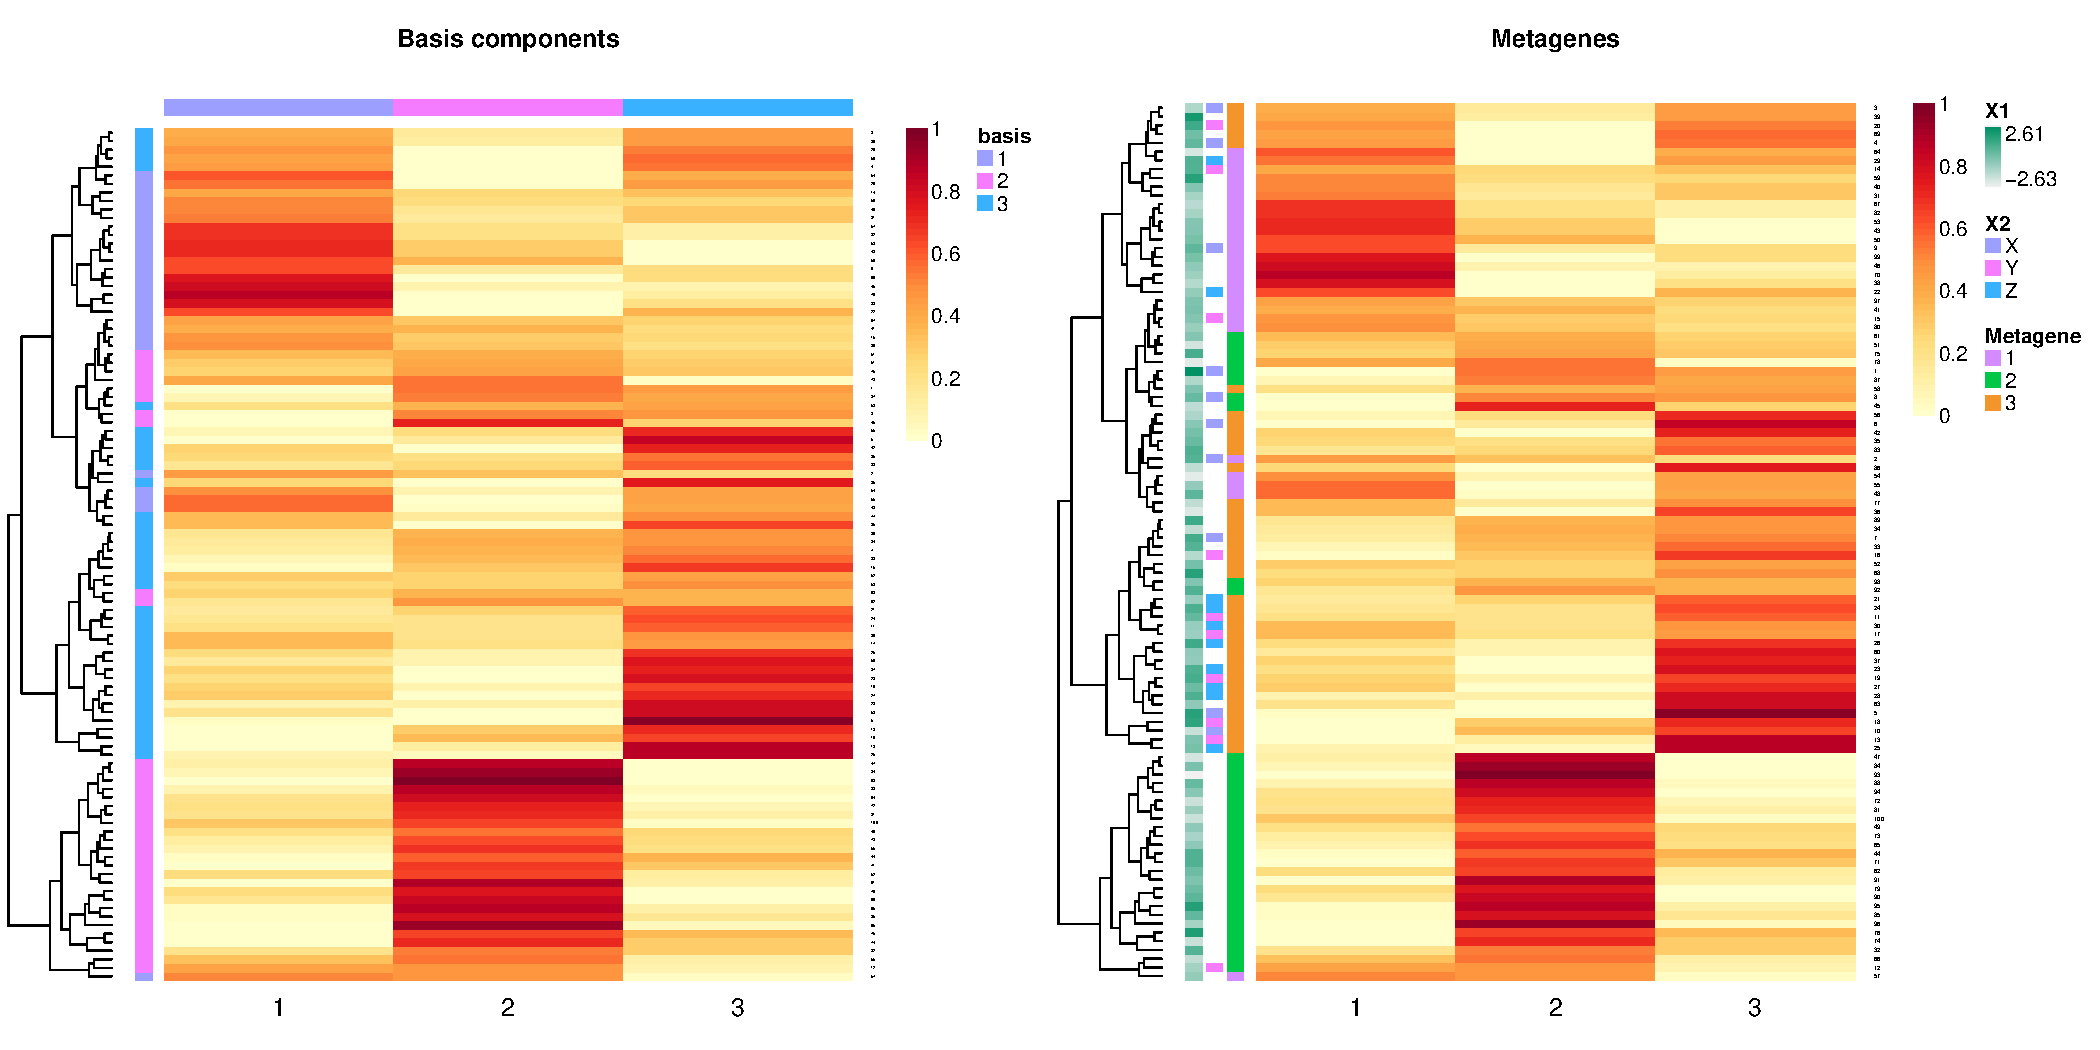
\includegraphics[width=\maxwidth]{/home/renaud/Documents/projects/NMF/pkg/vignettes/figure/heatmaps-basismap_res} 
\begin{kframe}\begin{alltt}
\hlfunctioncall{par}(opar)
\end{alltt}
\end{kframe}
\end{knitrout}


By default:
\begin{itemize}
\item the columns are not ordered;
\item the rows are ordered by hierarchical clustering using default distance and 
linkage methods (\code{'eculidean'} and \code{'complete'});
\item each row is scaled to sum up to one;
\item the color palette used is \code{'YlOrRd'} from the
\citeCRANpkg{RColorBrewer}, with 50 breaks.
\end{itemize}

In term of arguments passed to the heatmap engine \code{aheatmap}, these default 
settings translate as:

\begin{knitrout}
\definecolor{shadecolor}{rgb}{0.969, 0.969, 0.969}\color{fgcolor}\begin{kframe}
\begin{alltt}
Colv = NA
scale = \hlstring{"r1"}
color = \hlstring{"YlOrRd:50"}
annRow = \hlfunctioncall{predict}(object, \hlstring{"features"})
\end{alltt}
\end{kframe}
\end{knitrout}


\section{Consensus matrix: \texttt{consensusmap}}

When doing clustering with NMF, a common way of assessing the stability of the 
clusters obtained for a given rank is to consider the consensus matrix 
computed over multiple independent NMF runs, which is the average of the connectivity 
matrices of each separate run
\footnote{Hence, stability here means robustness with regards to the initial starting point, 
and shall not be interpreted as in e.g. cross-validation/bootstrap analysis. 
However, one can argue that having very consistent clusters across runs somehow supports 
for a certain regularity or the presence of an underlying pattern in the data.}.
This procedure is usually repeated over a certain range of factorization ranks, 
and the results are compared to identify which rank gives the best clusters, 
possibly in the light of some extra knowledge one could have about the samples 
(e.g. covariates).
The functions \code{nmf} and \code{consensusmap} make it easy to implement 
this whole process.

\nbnote{The consensus plots can also be generated for fits obtained from single NMF runs, 
in which case the consensus matrix simply reduces to a single connectivity matrix. 
This is a binary matrix (i.e. entries are either 0 or 1), that will always produce 
a bi-colour heatmap, and by default clear blocks for each cluster.}

\subsection{Single fit}
In section \cref{sec:data}, the NMF fit \code{res} was computed with argument 
\code{nrun=10}, and therefore contains the best fit over 10 runs, as well as 
the consensus matrix computed over all the runs
\footnote{If one were interested in keeping the fits from all the runs, the 
function \code{nmf} should have been called with argument \code{.options='k'}.
See section \emph{Options} in \code{?nmf}.
The downstream hanlding of the result would remain identical.}.
This can be ploted using the function \code{consensusmap}, which allows for the 
same kind of customization as the other NMF heatmap functions:

\begin{knitrout}
\definecolor{shadecolor}{rgb}{0.969, 0.969, 0.969}\color{fgcolor}\begin{kframe}
\begin{alltt}
opar <- \hlfunctioncall{par}(mfrow = \hlfunctioncall{c}(1, 2))
\hlcomment{# default plot}
\hlfunctioncall{consensusmap}(res)
\hlcomment{# customized plot}
\hlfunctioncall{consensusmap}(res, annCol = covariates, annColors = \hlfunctioncall{list}(c = \hlstring{"blue"}), labCol = \hlstring{"sample "}, 
    main = \hlstring{"Cluster stability"}, sub = \hlstring{"Consensus matrix and all covariates"})
\end{alltt}
\end{kframe}
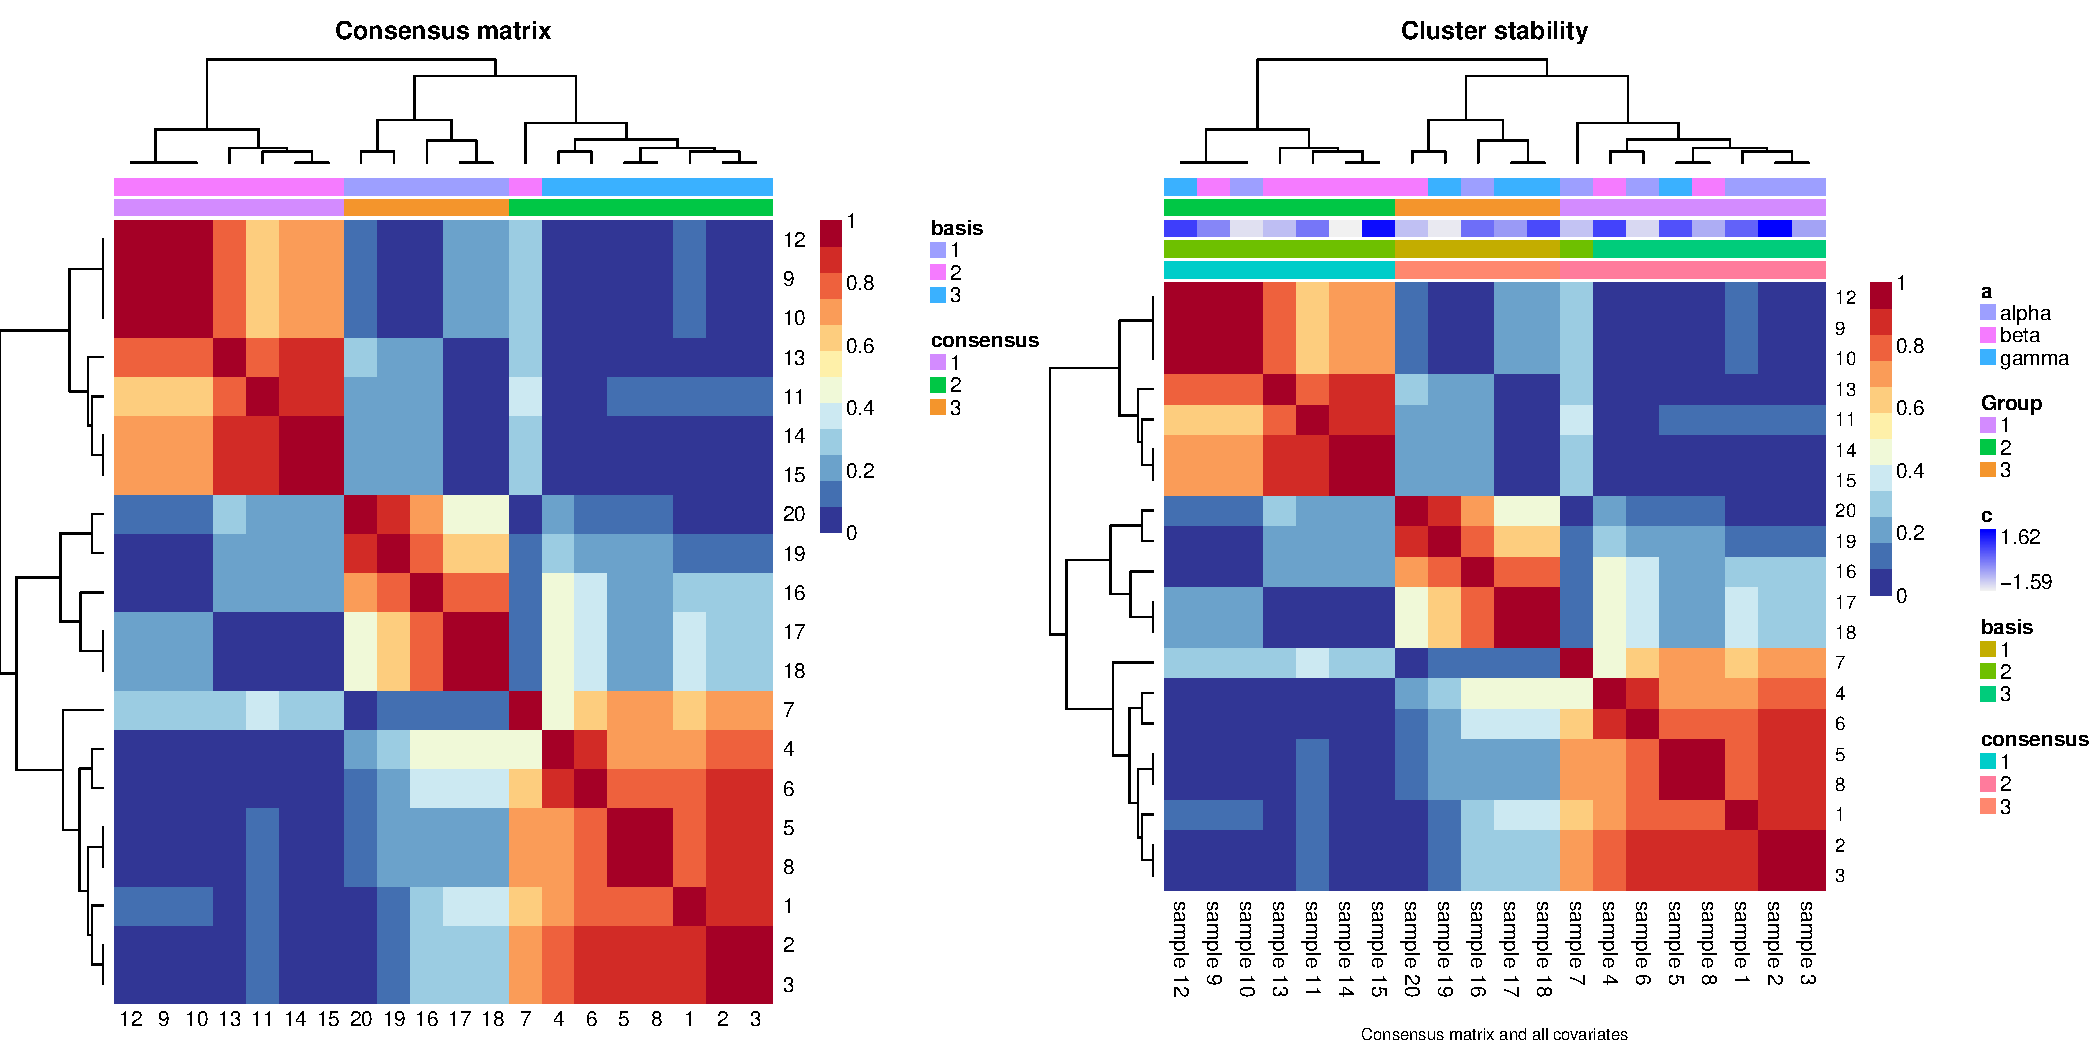
\includegraphics[width=\maxwidth]{/home/renaud/Documents/projects/NMF/pkg/vignettes/figure/heatmaps-consensusmap_res} 
\begin{kframe}\begin{alltt}
\hlfunctioncall{par}(opar)
\end{alltt}
\end{kframe}
\end{knitrout}


By default:
\begin{itemize}
\item the rows and columns of the consensus heatmap are symmetrically 
ordered by hierarchical clustering using the consensus matrix as a similarity 
measure and average linkage, and the associated dendrogram is displayed;
\item the color palette used is the reverse of \code{'RdYlBu'} from the \citeCRANpkg{RColorBrewer}.
\end{itemize}

In term of arguments passed to the heatmap engine \code{aheatmap}, these default 
settings translate as:

\begin{knitrout}
\definecolor{shadecolor}{rgb}{0.969, 0.969, 0.969}\color{fgcolor}\begin{kframe}
\begin{alltt}
distfun = \hlfunctioncall{function}(x) \hlfunctioncall{as.dist}(1 - x)  \hlcomment{# x being the consensus matrix}
hclustfun = \hlstring{"average"}
Rowv = TRUE
Colv = \hlstring{"Rowv"}
color = \hlstring{"-RdYlBu"}
\end{alltt}
\end{kframe}
\end{knitrout}


\subsection{Single method over a range of ranks}

The function \code{nmf} accepts a range of value for the rank (argument \code{rank}), 
making it fit NMF models for each value in the given range
\footnote{Before version 0.6, this feature was provided by the function \code{nmfEstimateRank}.
From version 0.6, the function \code{nmf} accepts ranges of ranks, and internally 
calls the function \code{nmfEstimateRank} -- that remains exported and can still 
be called directly. 
See documentation \code{?nmfEstimateRank} for more details on the returned value.}:

\begin{knitrout}
\definecolor{shadecolor}{rgb}{0.969, 0.969, 0.969}\color{fgcolor}\begin{kframe}
\begin{alltt}
res2_7 <- \hlfunctioncall{nmf}(X, 2:7, nrun = 10, .options = \hlstring{"v"})
\end{alltt}
\begin{verbatim}
## Compute NMF rank= 2  ... + measures ... OK
## Compute NMF rank= 3  ... + measures ... OK
## Compute NMF rank= 4  ... + measures ... OK
## Compute NMF rank= 5  ... + measures ... OK
## Compute NMF rank= 6  ... + measures ... OK
## Compute NMF rank= 7  ... + measures ... OK
\end{verbatim}
\begin{alltt}
\hlfunctioncall{class}(res2_7)
\end{alltt}
\begin{verbatim}
## [1] "NMF.rank"
\end{verbatim}
\end{kframe}
\end{knitrout}


The result \code{res2\_7} is an S3 object of class \code{'NMF.rank'}, 
that contains -- amongst other data -- a list of the best fits obtained for each 
value of the rank in range $\ldbrack 2, 7\rdbrack]$.
The method of \code{consensusmap} defined for class \code{'NMF.rank'}, 
which plots all the consensus matrices on the same plot: 

\begin{knitrout}
\definecolor{shadecolor}{rgb}{0.969, 0.969, 0.969}\color{fgcolor}\begin{kframe}
\begin{alltt}
\hlfunctioncall{consensusmap}(res2_7)
\end{alltt}
\end{kframe}
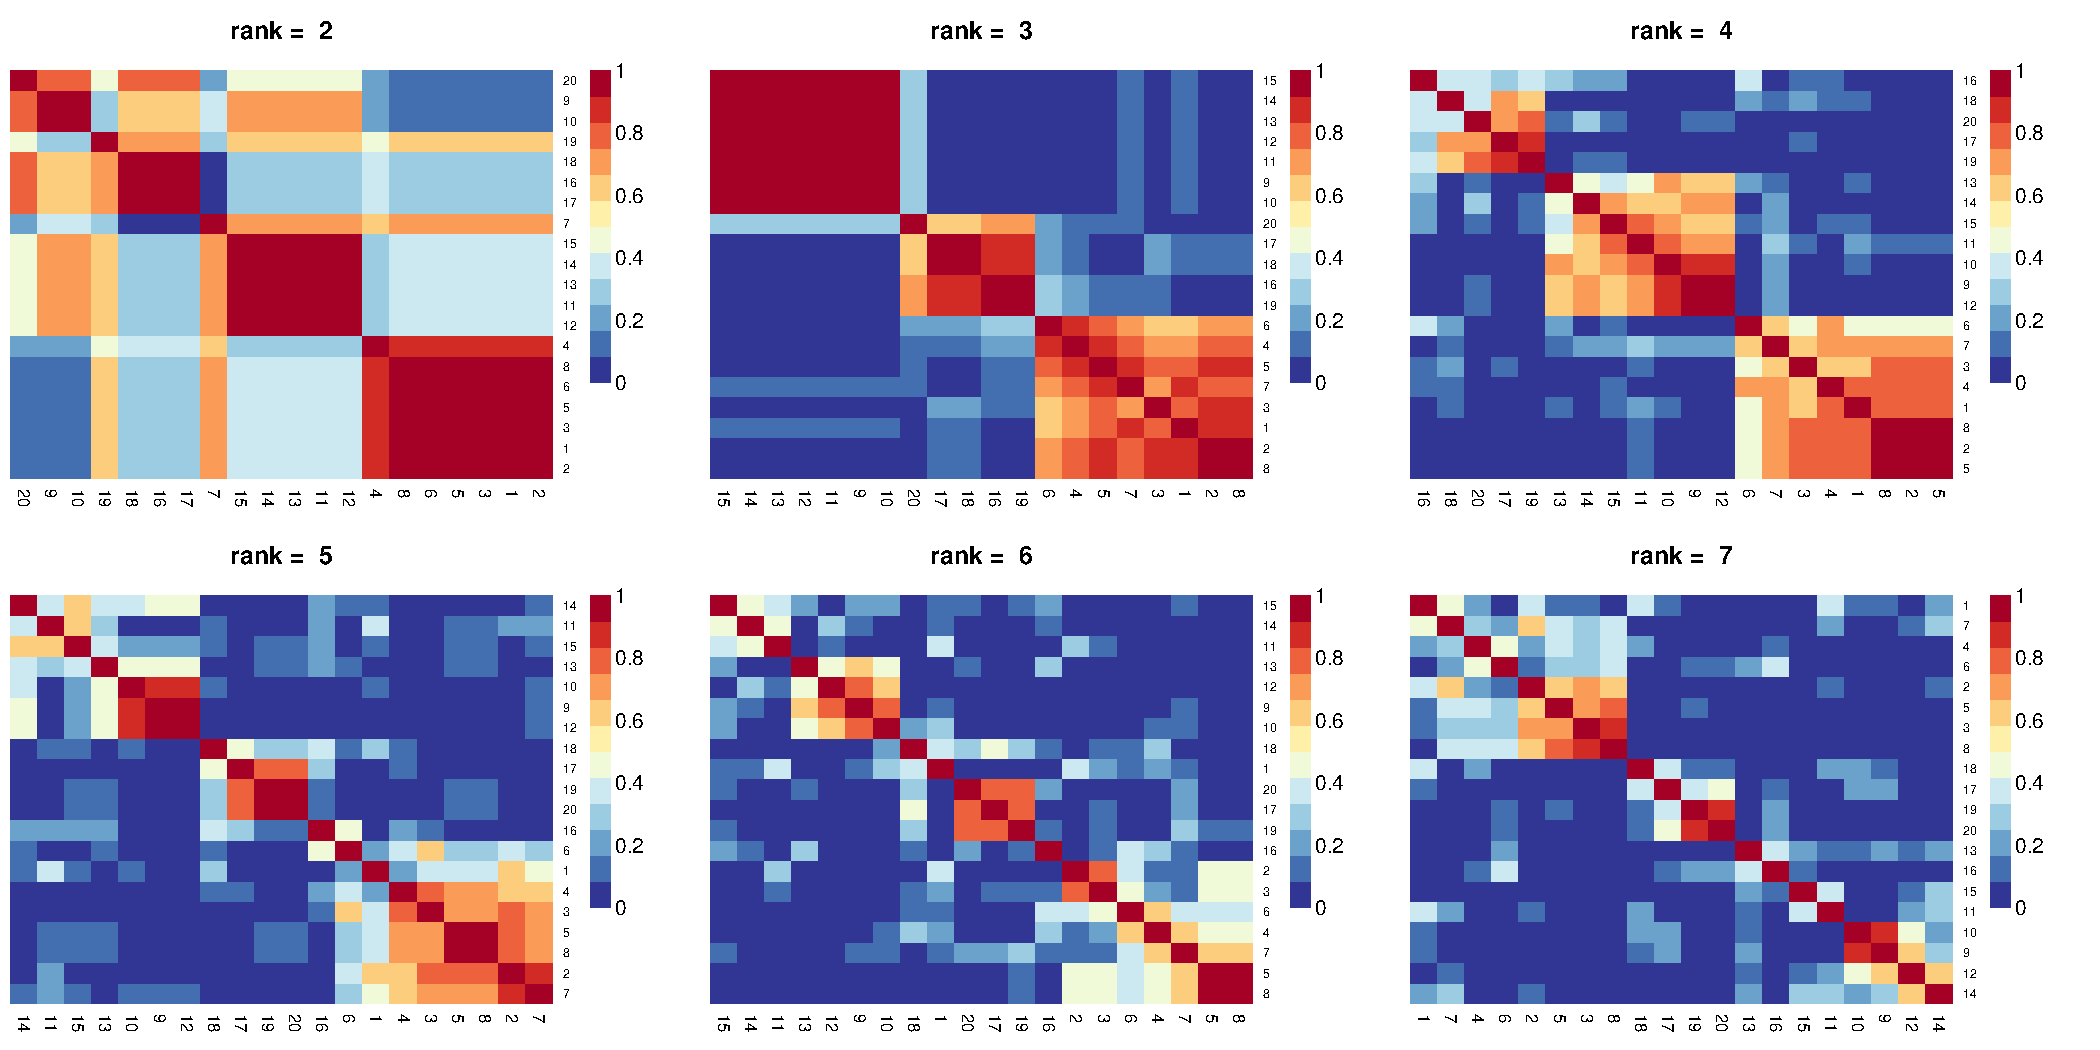
\includegraphics[width=\maxwidth]{/home/renaud/Documents/projects/NMF/pkg/vignettes/figure/heatmaps-consensusmap_estimate} 

\end{knitrout}


\nbnote{ The main title of each consensus heatmap can be customized by passing 
to argument \code{main} a character vector or a list whose elements specify each title.
All other arguments are used in each internal call to consensusmap, and will 
therefore affect all the plots simultaneously.
The layout can be specified via argument \code{layout} as a numeric vector 
giving the number of rows and columns in a \code{mfrow}-like way, or as a 
matrix that will be passed to R core function \code{layout}.
See \code{?consensusmap} for more details and example code.
}

\subsection{Single rank over a range of methods}
If one is interested in comparing methods, for a given factorization rank, then 
on can fit an NMF model for each method by providing the function \code{nmf} with 
a \code{list} in argument \code{method}:

\begin{knitrout}
\definecolor{shadecolor}{rgb}{0.969, 0.969, 0.969}\color{fgcolor}\begin{kframe}
\begin{alltt}
res_methods <- \hlfunctioncall{nmf}(X, 3, \hlfunctioncall{list}(\hlstring{"lee"}, \hlstring{"brunet"}, \hlstring{"nsNMF"}), nrun = 10)
\end{alltt}
\begin{verbatim}
## Compute NMF method 'lee' [1/3] ... OK
## Compute NMF method 'brunet' [2/3] ... OK
## Compute NMF method 'nsNMF' [3/3] ... OK
\end{verbatim}
\begin{alltt}
\hlfunctioncall{class}(res_methods)
\end{alltt}
\begin{verbatim}
## [1] "NMFList"
## attr(,"package")
## [1] "NMF"
\end{verbatim}
\end{kframe}
\end{knitrout}


The result \code{res\_methods} is an S4 object of class \code{NMFList}, which 
is essentially a named list, that contains each fits and the CPU time required 
by the whole computation.
As previously, the sequence of consensus matrices is plotted with \code{consensusmap}:

\begin{knitrout}
\definecolor{shadecolor}{rgb}{0.969, 0.969, 0.969}\color{fgcolor}\begin{kframe}
\begin{alltt}
\hlfunctioncall{consensusmap}(res_methods)
\end{alltt}
\end{kframe}
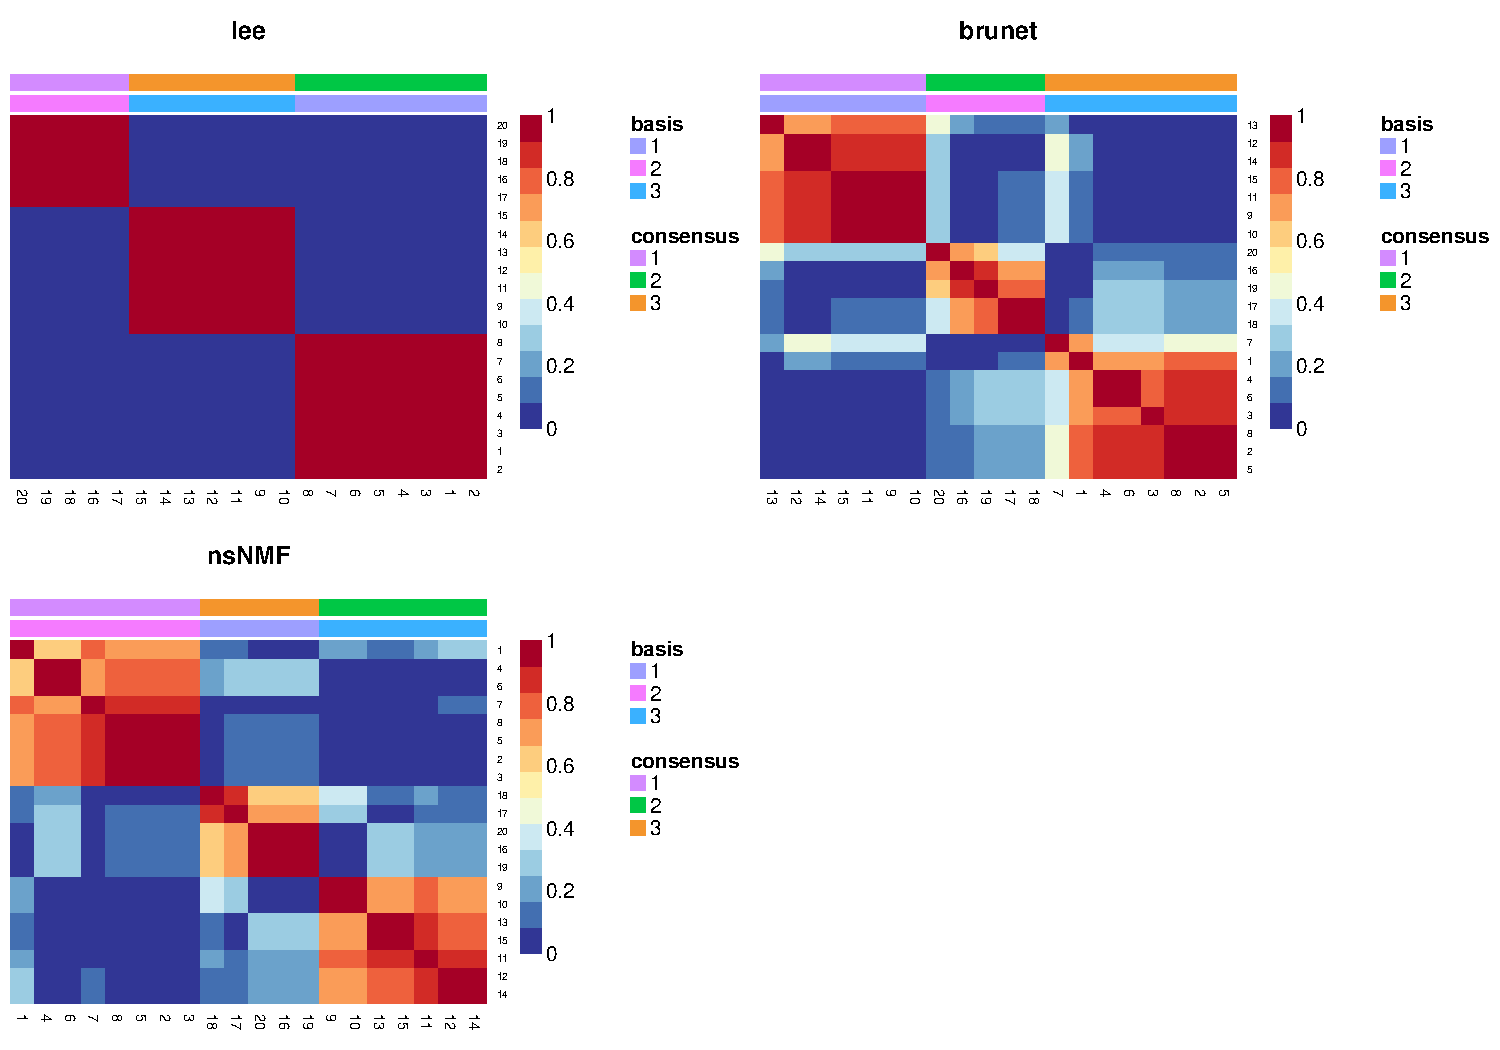
\includegraphics[width=\maxwidth]{/home/renaud/Documents/projects/NMF/pkg/vignettes/figure/heatmaps-consensusmap_methods} 

\end{knitrout}


\section{Generic heatmap engine: \texttt{aheatmap}}
\label{sec:aheatmap}

This section still needs to be written, but many examples of annotated heatmaps can be found in the demos \code{'aheatmap'} and \code{'heatmaps'}:
\begin{knitrout}
\definecolor{shadecolor}{rgb}{0.969, 0.969, 0.969}\color{fgcolor}\begin{kframe}
\begin{alltt}
\hlfunctioncall{demo}(\hlstring{"aheatmap"})
\hlcomment{# or}
\hlfunctioncall{demo}(\hlstring{"heatmaps"})
\end{alltt}
\end{kframe}
\end{knitrout}


These demos and the plots they generate can also be browsed online at \url{http://nmf.r-forge.r-project.org/_DEMOS.html}.

\section{Session Info}
\begin{itemize}\raggedright
  \item R version 2.15.2 (2012-10-26), \verb|i686-pc-linux-gnu|
  \item Locale: \verb|LC_CTYPE=en_US.UTF-8|, \verb|LC_NUMERIC=C|, \verb|LC_TIME=en_US.UTF-8|, \verb|LC_COLLATE=en_US.UTF-8|, \verb|LC_MONETARY=en_US.UTF-8|, \verb|LC_MESSAGES=en_US.UTF-8|, \verb|LC_PAPER=C|, \verb|LC_NAME=C|, \verb|LC_ADDRESS=C|, \verb|LC_TELEPHONE=C|, \verb|LC_MEASUREMENT=en_US.UTF-8|, \verb|LC_IDENTIFICATION=C|
  \item Base packages: base, datasets, graphics, grDevices, grid,
    methods, stats, utils
  \item Other packages: bigmemory~4.3.0, bigmemory.sri~0.1.2,
    Biobase~2.18.0, BiocGenerics~0.4.0, digest~0.6.3, knitr~1.1,
    NMF~0.11, pkgmaker~0.12, RColorBrewer~1.0-5, registry~0.2,
    rngtools~1.1.2, synchronicity~1.1.0
  \item Loaded via a namespace (and not attached):
    codetools~0.2-8, colorspace~1.2-1, doParallel~1.0.1,
    evaluate~0.4.3, foreach~1.4.0, formatR~0.7, gridBase~0.4-6,
    iterators~1.0.6, stringr~0.6.2, tools~2.15.2, xtable~1.7-1
\end{itemize}



\printbibliography[heading=bibintoc]


\end{document}
